%%%%%%%%%%%%%%%%%%%%%%%%%%% asme2ej.tex %%%%%%%%%%%%%%%%%%%%%%%%%%%%%%%
% Template for producing ASME-format journal articles using LaTeX    %
% Written by   Harry H. Cheng, Professor and Director                %
%              Integration Engineering Laboratory                    %
%              Department of Mechanical and Aeronautical Engineering %
%              University of California                              %
%              Davis, CA 95616                                       %
%              Tel: (530) 752-5020 (office)                          %
%                   (530) 752-1028 (lab)                             %
%              Fax: (530) 752-4158                                   %
%              Email: hhcheng@ucdavis.edu                            %
%              WWW:   http://iel.ucdavis.edu/people/cheng.html       %
%              May 7, 1994                                           %
% Modified: February 16, 2001 by Harry H. Cheng                      %
% Modified: January  01, 2003 by Geoffrey R. Shiflett                %
% Butchered: October 15, 2014 by John Karasinski                     %
% Use at your own risk, send complaints to /dev/null                 %
%%%%%%%%%%%%%%%%%%%%%%%%%%%%%%%%%%%%%%%%%%%%%%%%%%%%%%%%%%%%%%%%%%%%%%

%%% use twocolumn and 10pt options with the asme2ej format
\documentclass[twocolumn,10pt]{asme2ej}

\usepackage{epsfig} %% for loading postscript figures
\usepackage{amsmath}
\usepackage{graphicx}
\usepackage{grffile}
\usepackage{pdfpages}
\usepackage{algpseudocode}
\usepackage{subcaption}

% Default fixed font does not support bold face
\DeclareFixedFont{\ttb}{T1}{txtt}{bx}{n}{12} % for bold
\DeclareFixedFont{\ttm}{T1}{txtt}{m}{n}{12}  % for normal

% Custom colors
\usepackage{color}
\usepackage{listings}
\usepackage{framed}
\usepackage{caption}
\captionsetup[lstlisting]{font={small,tt}}

\definecolor{mygreen}{rgb}{0,0.6,0}
\definecolor{mygray}{rgb}{0.5,0.5,0.5}
\definecolor{mymauve}{rgb}{0.58,0,0.82}

\lstset{ %
  backgroundcolor=\color{white},   % choose the background color; you must add \usepackage{color} or \usepackage{xcolor}
  basicstyle=\ttfamily\footnotesize, % the size of the fonts that are used for the code
  breakatwhitespace=false,         % sets if automatic breaks should only happen at whitespace
  % breaklines=true,                 % sets automatic line breaking
  captionpos=b,                    % sets the caption-position to bottom
  commentstyle=\color{mygreen},    % comment style
  deletekeywords={...},            % if you want to delete keywords from the given language
  escapeinside={\%*}{*)},          % if you want to add LaTeX within your code
  extendedchars=true,              % lets you use non-ASCII characters; for 8-bits encodings only, does not work with UTF-8
  frame=single,                    % adds a frame around the code
  keepspaces=true,                 % keeps spaces in text, useful for keeping indentation of code (possibly needs columns=flexible)
  columns=flexible,
  keywordstyle=\color{blue},       % keyword style
  language=Python,                 % the language of the code
  morekeywords={*,...},            % if you want to add more keywords to the set
  numbers=left,                    % where to put the line-numbers; possible values are (none, left, right)
  numbersep=5pt,                   % how far the line-numbers are from the code
  numberstyle=\tiny\color{mygray}, % the style that is used for the line-numbers
  rulecolor=\color{black},         % if not set, the frame-color may be changed on line-breaks within not-black text (e.g. comments (green here))
  showspaces=false,                % show spaces everywhere adding particular underscores; it overrides 'showstringspaces'
  showstringspaces=false,          % underline spaces within strings only
  showtabs=false,                  % show tabs within strings adding particular underscores
  stepnumber=1,                    % the step between two line-numbers. If it's 1, each line will be numbered
  stringstyle=\color{mymauve},     % string literal style
  tabsize=4,                       % sets default tabsize to 2 spaces
}

\title{Final: Incompressible, Laminar Flow over a Rectangular Cavity}

\author{John Karasinski
    \affiliation{
  Graduate Student Researcher\\
  Center for Human/Robotics/Vehicle Integration and Performance\\
  Department of Mechanical and Aerospace Engineering\\
  University of California\\
  Davis, California 95616\\
    Email: karasinski@ucdavis.edu
    }
}

\begin{document}
\maketitle

%%%%%%%%%%%%%%%%%%%%%%%%%%%%%%%%%%%%%%%%%%%%%%%%%%%%%%%%%%%%%%%%%%%%%%
\section{Problem Description}

Forty five years ago, Mehta and Lavan published a paper on the numerical investigation of flow over a rectangular cavity at low Reynolds numbers~\cite{mehta1969flow}. This relatively simple geometry provides tremendous insight into the physics of flow separation, an important flow feature in many applications. A numerical 2D planar model of these incompressible, laminar flows is developed here. In particular, the predicted flow structure (streamline pattern, eddies) and velocity profiles are investigated for a variety of aspect ratios (AR) and Reynolds numbers (Re).

\begin{figure}[b]
\begin{center}
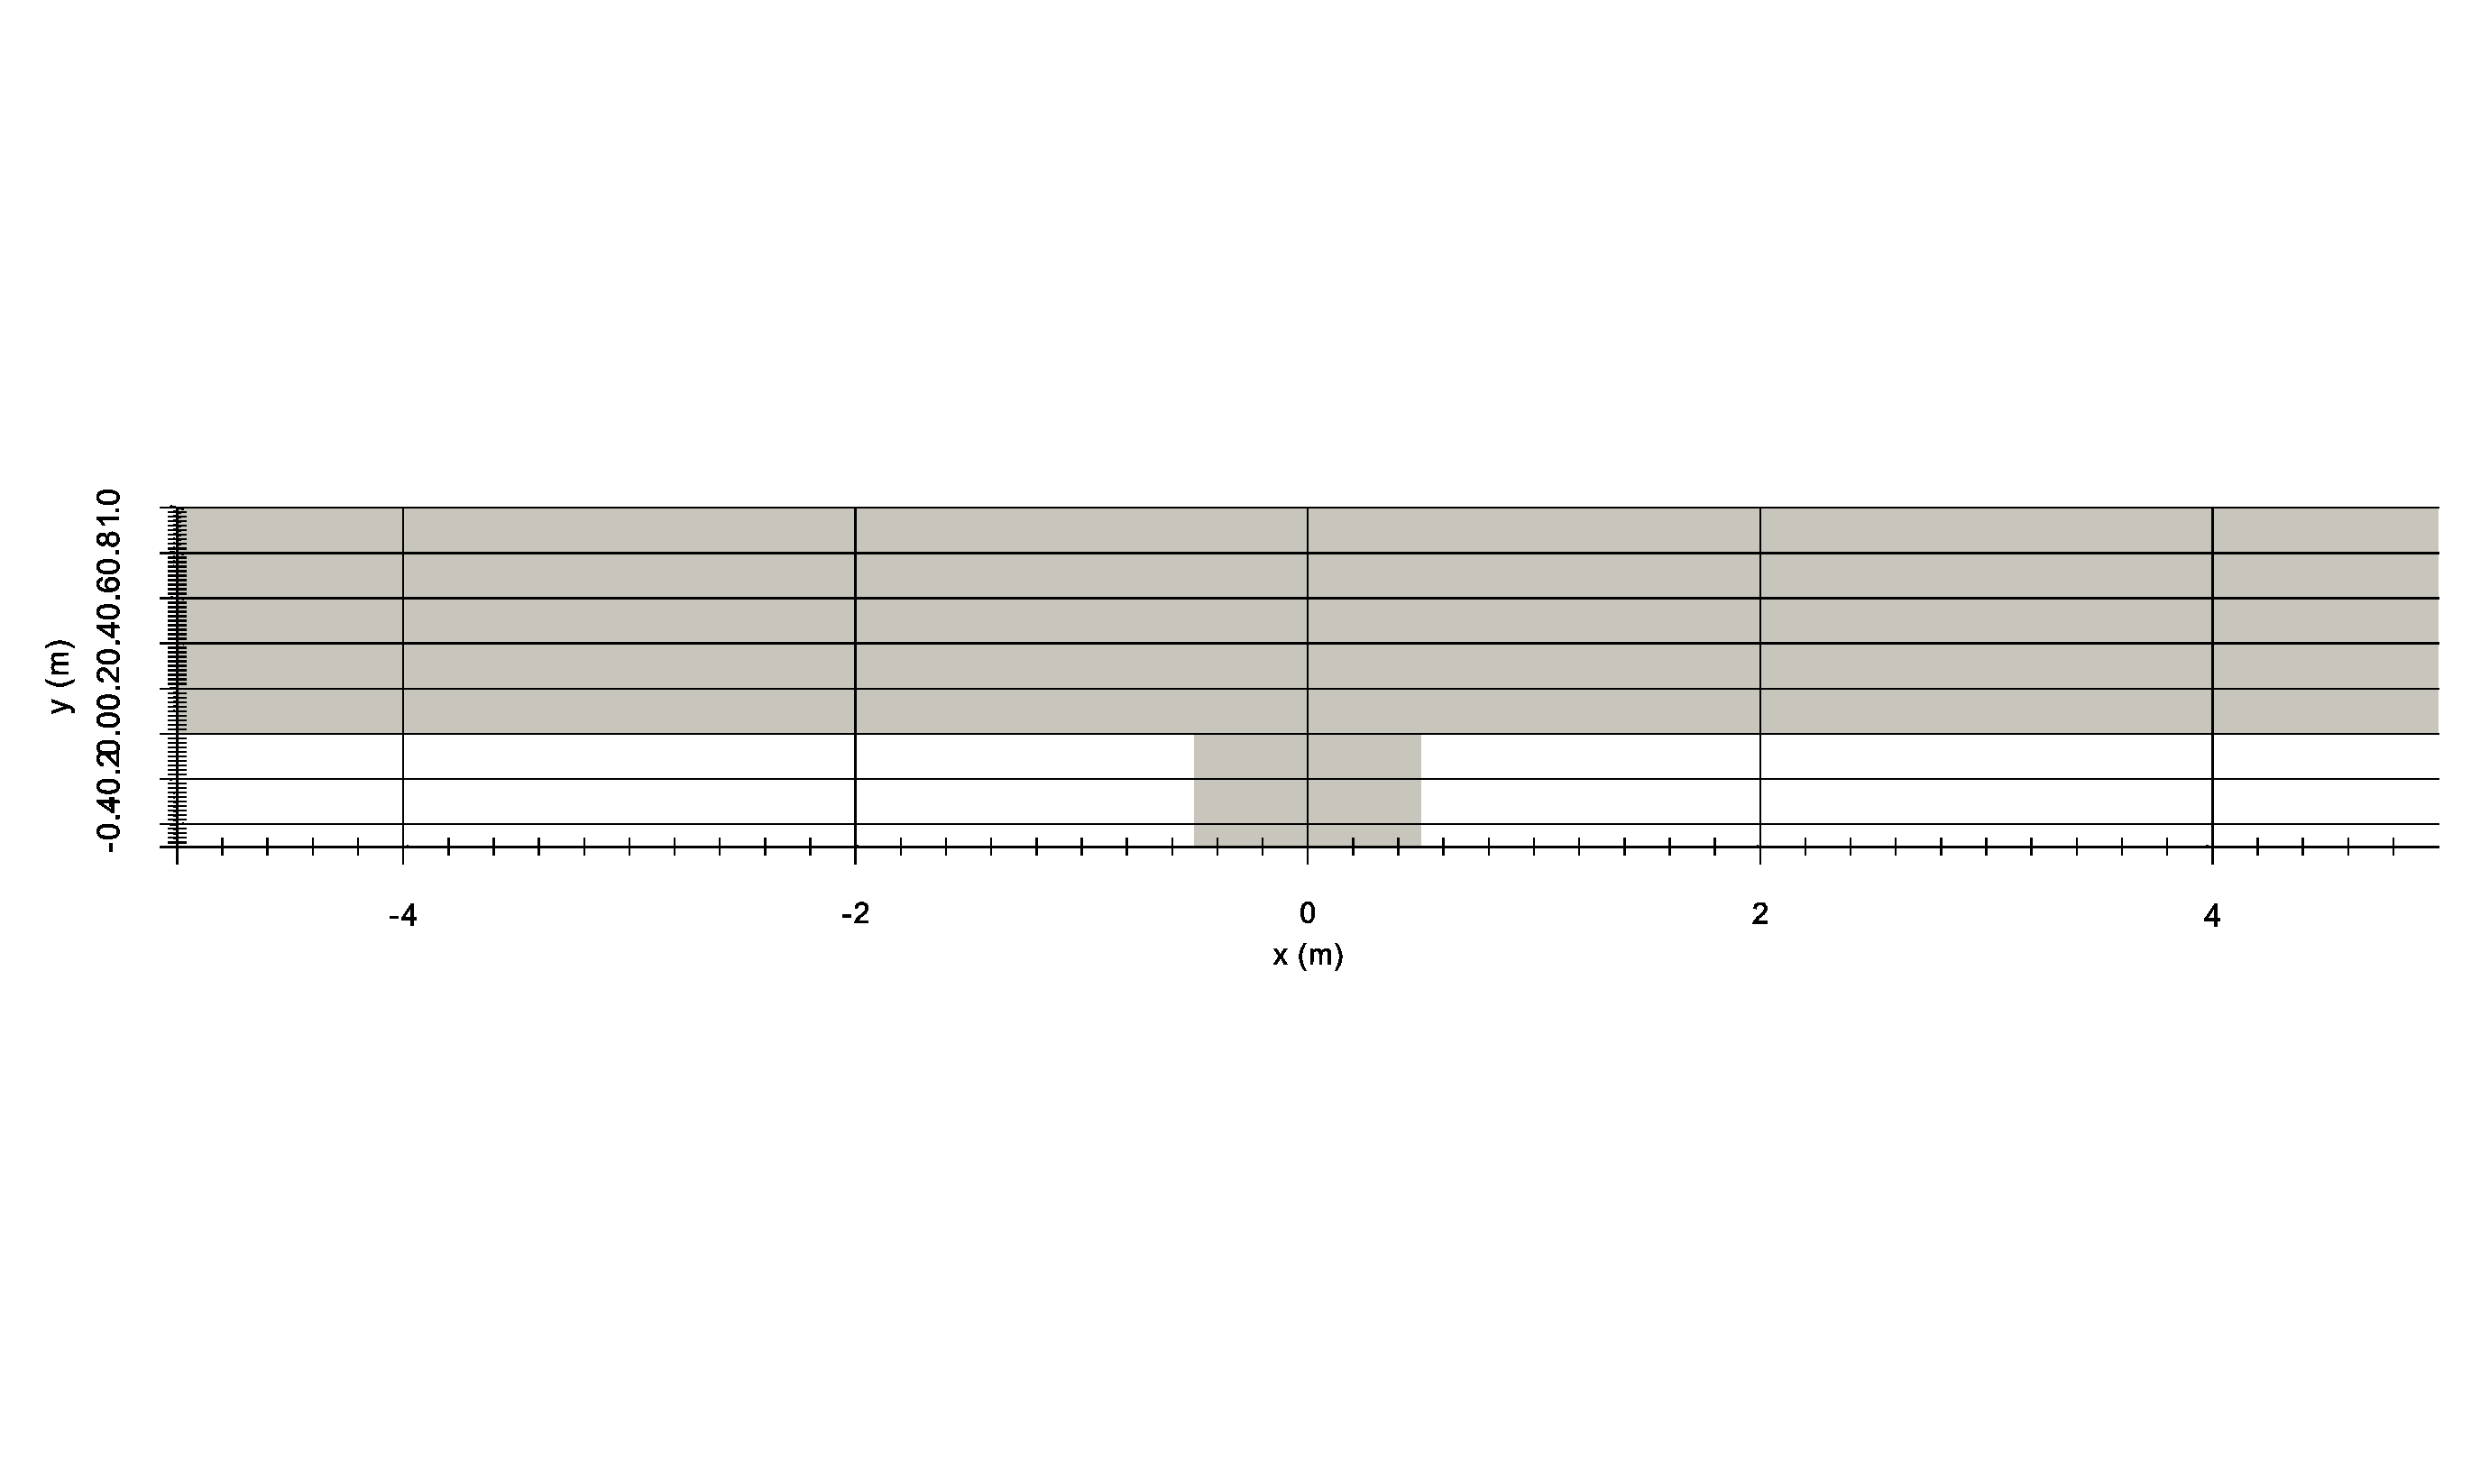
\includegraphics[width=0.5\textwidth]{figure/geometry.pdf}
\caption{Geometry for the AR=0.5 cases (width of channel = 10m, height of channel = 1m; width of cavity = 1m, height of channel = 0.5m)}
\label{geometry_figure}
\end{center}
\end{figure}

%%%%%%%%%%%%%%%%%%%%%%%%%%%%%%%%%%%%%%%%%%%%%%%%%%%%%%%%%%%%%%%%%%%%%%
\section{Numerical Solution Approach}

The icoFoam solver from OpenFOAM 2.3.0 was used to computationally solve the Navier-Stokes equations,
\begin{equation}
\rho \left(\frac{\partial \mathbf{v}}{\partial t} + \mathbf{v} \cdot \nabla \mathbf{v}\right) = -\nabla p + \mu \nabla^2 \mathbf{v} + \mathbf{f}.
\end{equation}
\noindent icoFoam is a transient solver for incompressible, laminar flow of Newtonian fluid. The geometry for this problem consists of a channel of width 10 m and height 1 m. A cavity is placed just below the center of this channel and has a width of 1 m and a depth of AR (see Figure~\ref{geometry_figure}). Five cases were investigated: a base case with AR=0.5 and Re=100, and additional cases of AR=0.5 with Re=1 and 2000 for AR=0.5, and AR=2.0 and 5.0 for Re=100. A Python script was created to generate the initial conditions, geometry, and meshes for each case.

\subsection{Initial and Boundary Conditions}
The initial velocity field is set to zero throughout the domain. Additionally, the top lid of the channel is set to move to the right at 1 m/s and the velocity at the walls is set to zero. The initial pressure field is also set to zero throughout the domain, and the lid and walls are set to a ``zeroGradient'' condition. The boundary field for the inlet and outlet boundaries are set to ``zeroGradient'' for all of the initial fields, and the boundary field for frontAndBack is set to ``empty'' for all initial fields, turning this into a 2D problem.

\subsection{Geometry and Mesh}
The script also generated the nonuniform mesh for this geometry using the\lstinline{blockMesh} tool. This mesh was divided into four blocks: the left half of the channel, the right half of the channel, the center of the channel, and the cavity. For the base case, both the left and right halves of the channel were split into 100x100 points in the x, y direction, and also used ``simpleGrading'' in the x-direction to grade the meshes to be denser towards the center of the domain. The center of the channel was also split into 100x100 points in the x, y direction. The cavity for the base case was split into 100x50 points in the x, y direction. A generalized version of this mesh is available in Table~\ref{mesh_generation} (where M is some desired mesh size).

The resulting mesh was then split on to four CPUs using the\lstinline{decomposePar} tool, and the icoFoam solver was called with the MPI option. The solver than solved the system to the specified end time and reconstructed the domain and fields using the\lstinline{reconstructPar} tool. Solving to a solution time of 10 seconds for the base case takes 92.82s on a single core and only 44.01s on four cores, leading to a speedup of 2.1. This speedup could likely be improved by changing the distribution of the mesh onto the processors.

\begin{table}[tb]
\begin{center}
\begin{tabular}{| l | r r r | }
\hline
Name            & x &  y    & simpleGrading \\
\hline
Left channel    & M &  M    & (5/M 1 1) \\
Right channel   & M &  M    & (M/5 1 1) \\
Central channel & M &  M    & (1   1 1) \\
Cavity          & M &  M*AR & (1   1 1) \\
\hline
\end{tabular}
\caption{Mesh configuration algorithm (M=100, AR=0.5 for base case)}
\label{mesh_generation}
\end{center}
\end{table}

%%%%%%%%%%%%%%%%%%%%%%%%%%%%%%%%%%%%%%%%%%%%%%%%%%%%%%%%%%%%%%%%%%%%%%
\section{Results Discussion}
\subsection{Comparison to Previously Published Results}

\subsection{Velocity Profile Convergence}
The system was considered converged when the velocity profile before and after the cavity both approximated a linear function. This is accomplished by sampling the velocity profile at x = 1 m and x = -1 m with the\lstinline{sample} tool and plotting against y. An example of this velocity profile for the base case at $t=30$s can be seen in Figure~\ref{velocity_profile}.

The NRMS as a function of time is also investigated. A linear velocity profile was taken as the exact solution, and was used as the basis for comparison between the computational solutions found at each time step. The Root Mean Square error,
\begin{equation}
RMSE = \sqrt{\frac{1}{N}\sum\limits_{i=1}^N[U_i - U^*]^2},
\end{equation}
and the Normalized Root Mean Square error,
\begin{equation}
NRMS = \dfrac{RMSE}{max(U^*)-min(U^*)},
\end{equation}
can be calculated (as $max(U^*)-min(U^*) = 1$ in this case, the $NRMS = RMS$). Here $U_i$ is the computational result at each sampled point, $U^*$ is the linear velocity profile solution, and $N$ is the number of sampled points. The $NRMS$ for each case is expressed as a percentage, where lower values indicate a result closer to the analytic solution.

The results of NRMS of the base case at each time step for the velocity profiles before and after the cavity are plotted in Figure~\ref{convergence_plot}. This shows that the convergence of the velocity profile after the cavity converges to $NRMS \approx 2E-4$ at approximately $t=120$s, while the velocity profile before the cavity continues to decrease logarithmically. The convergence of the velocity profile after the cavity suggests that the vortices in the cavity are also effectively converged by this time.

\begin{figure}[tbh]
\begin{center}
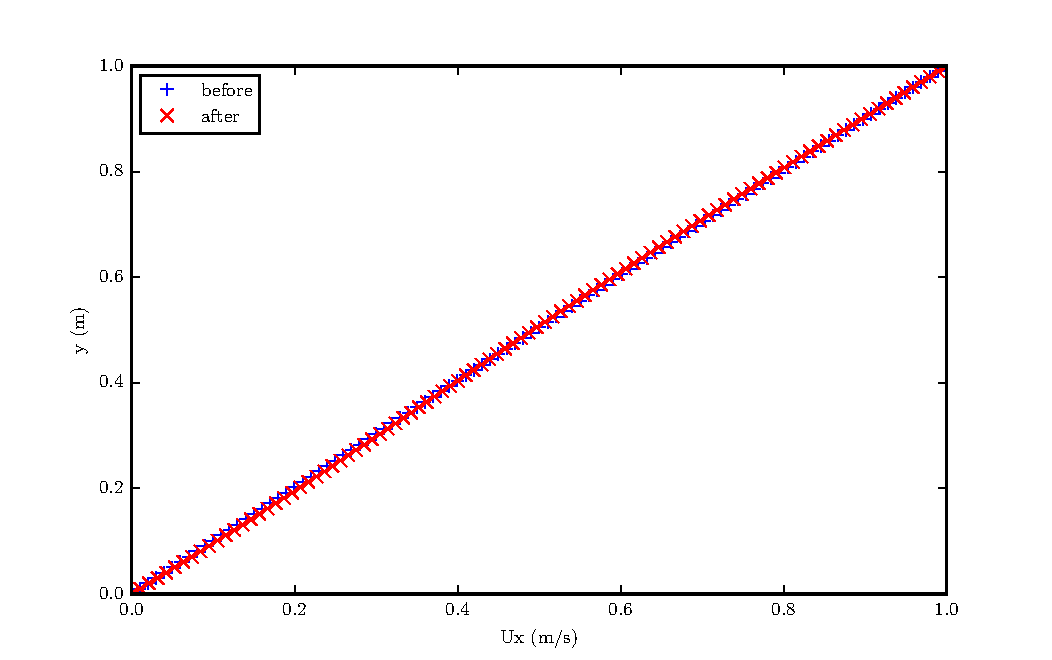
\includegraphics[width=0.5\textwidth]{figure/Ar0.5-Re100 Ux before and after.pdf}
\caption{Velocity profile of Ux before ($x = 1 $m) and after ($x = -1 $m) cavity, for base case at $t=30$s}
\label{velocity_profile}
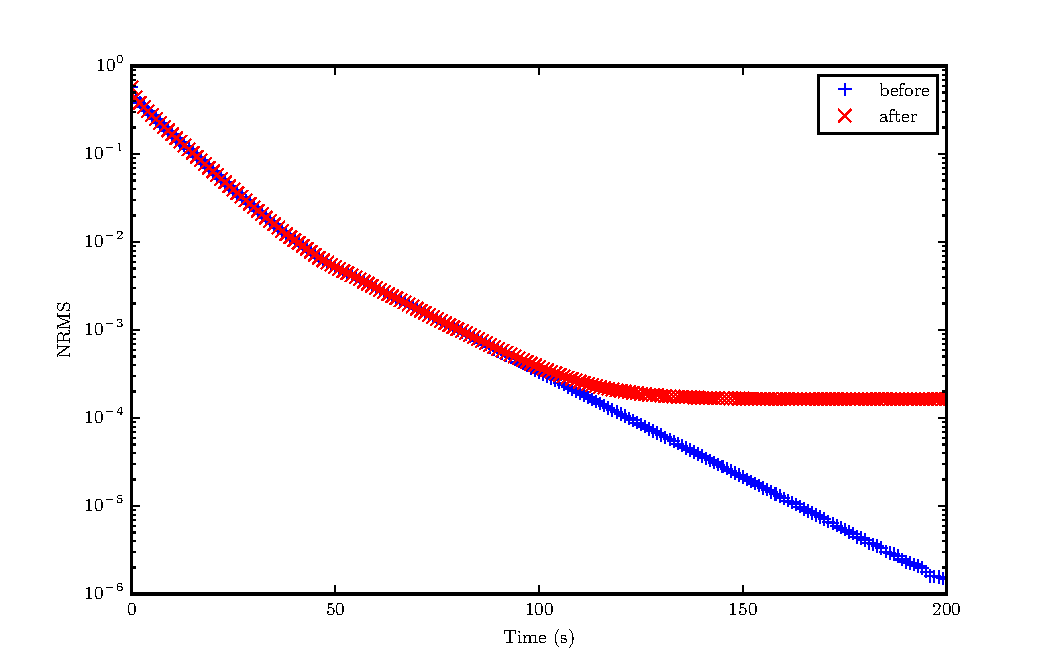
\includegraphics[width=0.5\textwidth]{figure/convergence.pdf}
\caption{Convergence of velocity profile before ($x = 1 $m) and after ($x = -1 $m) cavity, for base case}
\label{convergence_plot}
\end{center}
\end{figure}

\begin{figure}[tbh]
\begin{center}
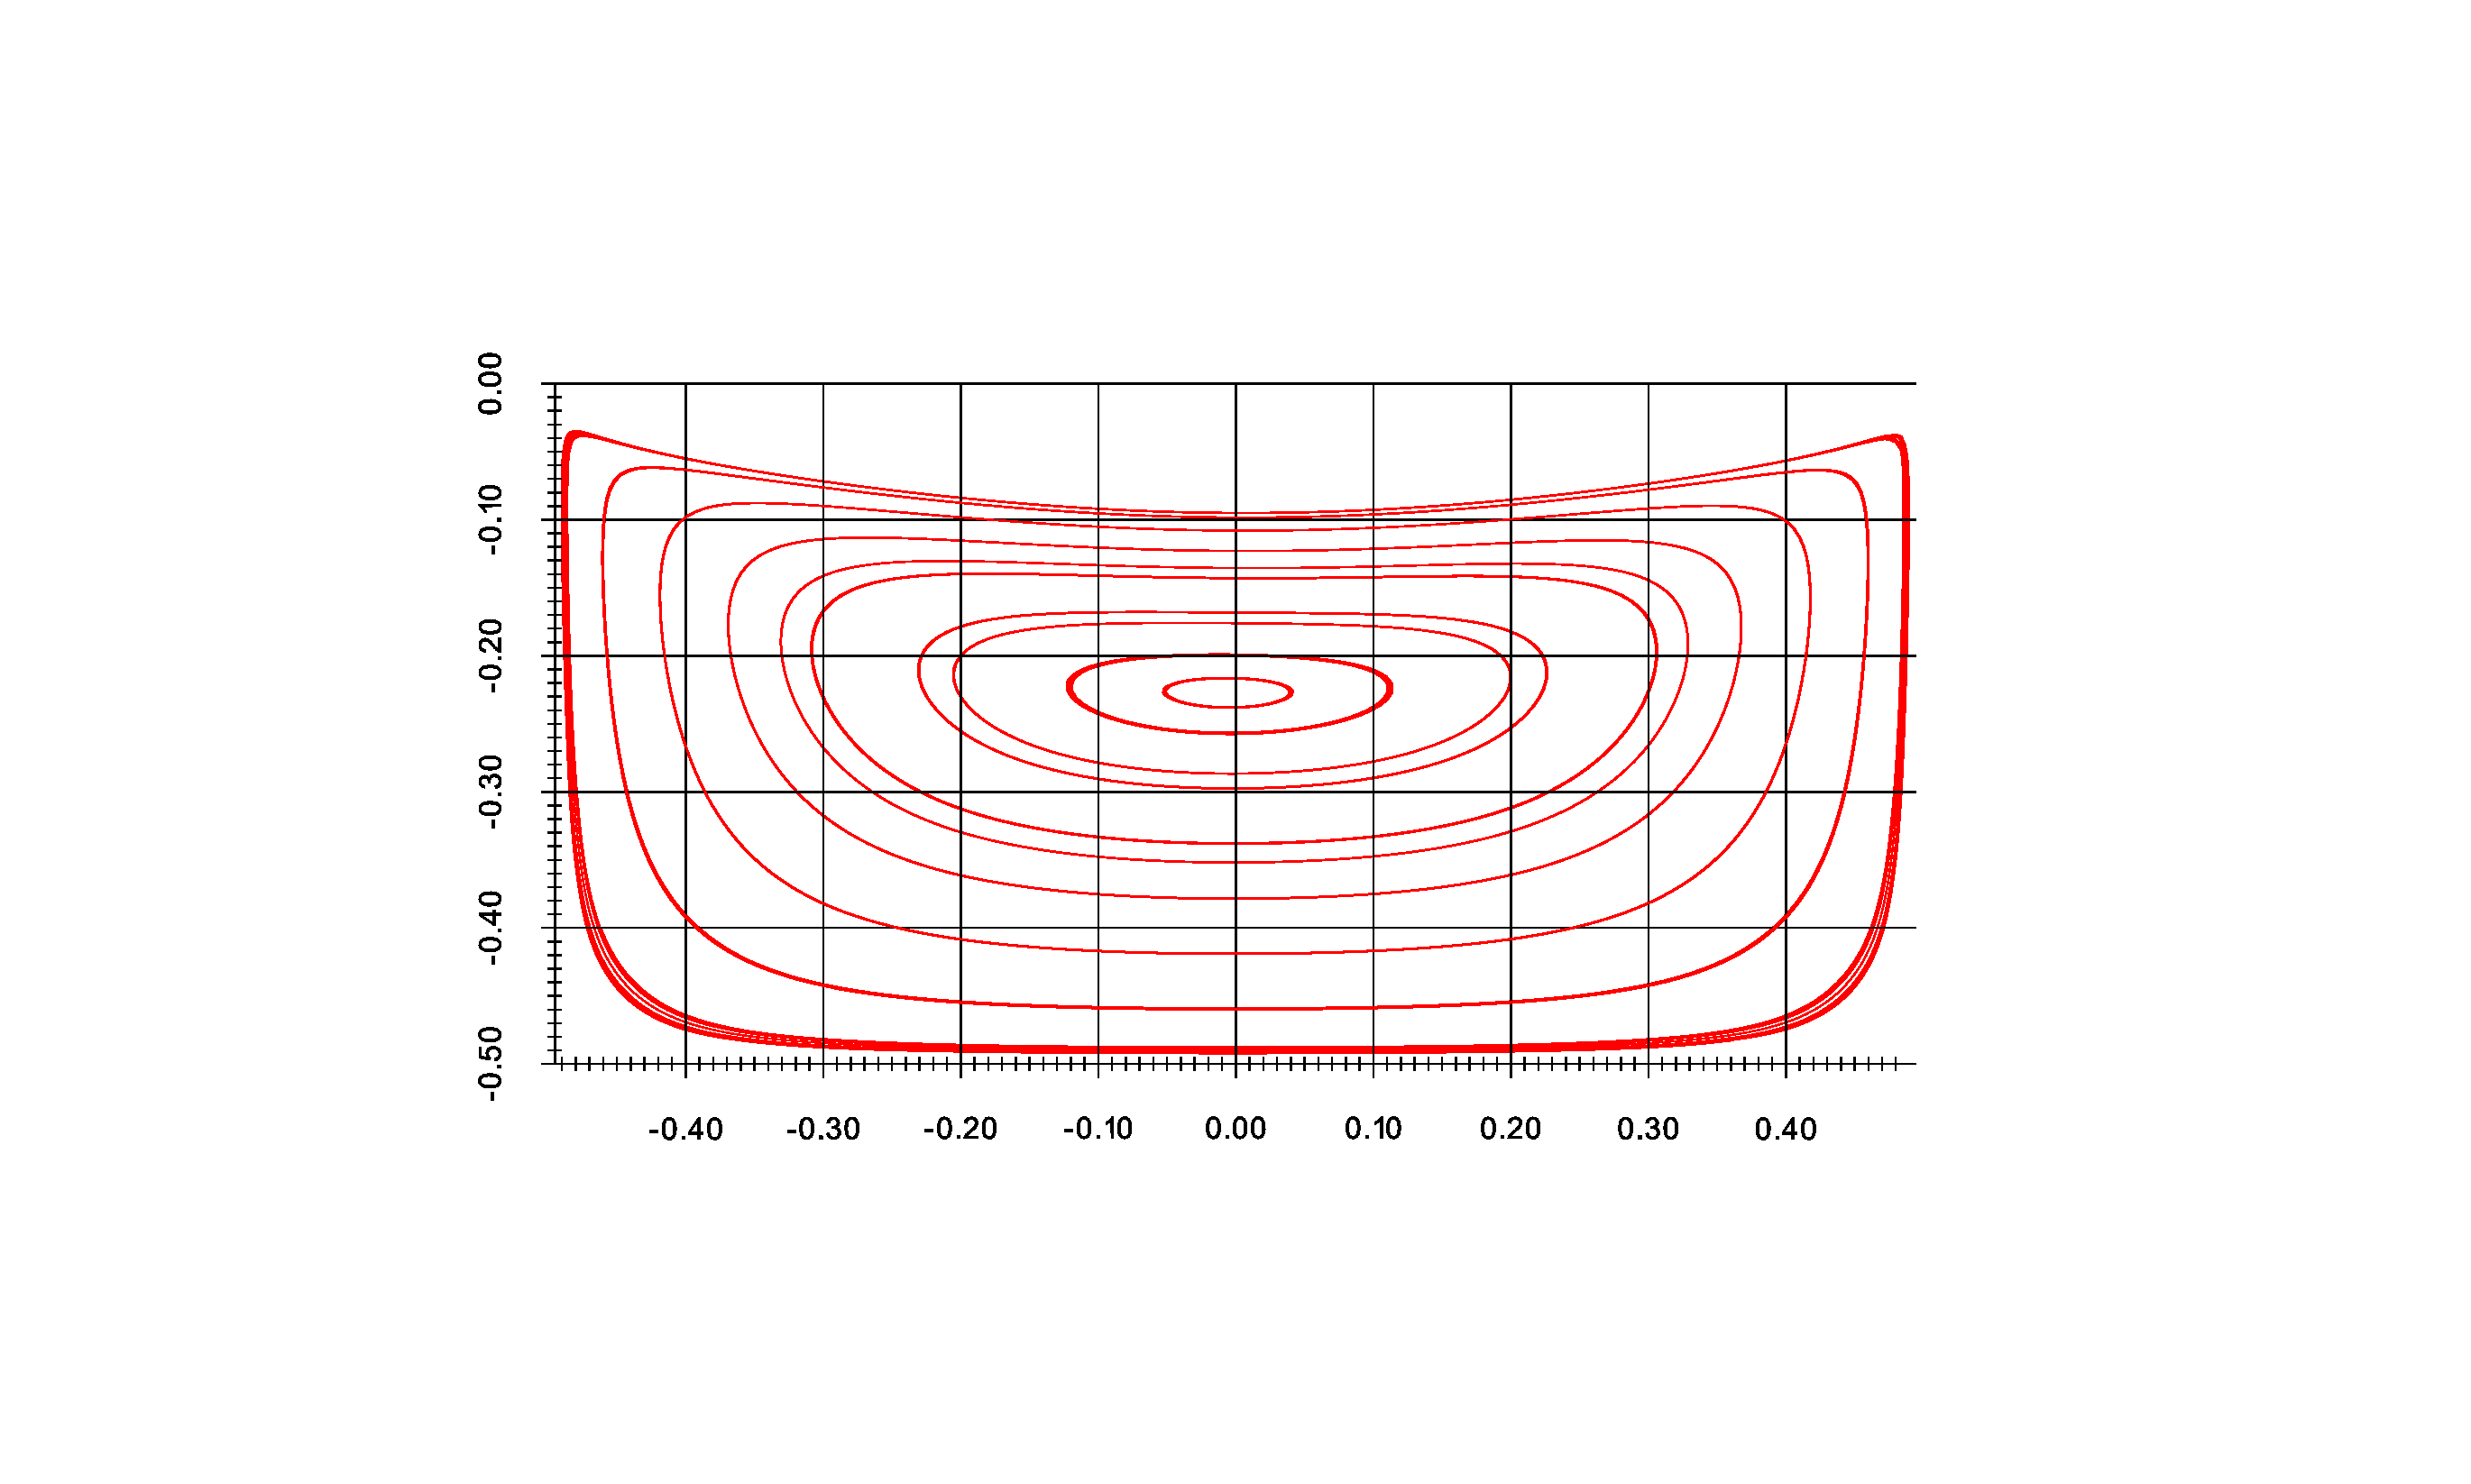
\includegraphics[width=0.5\textwidth]{figure/AR0.5-Re1 streamFunction axis final.pdf}
\caption{AR=0.5, Re=1}
\label{AR0.5RE1}

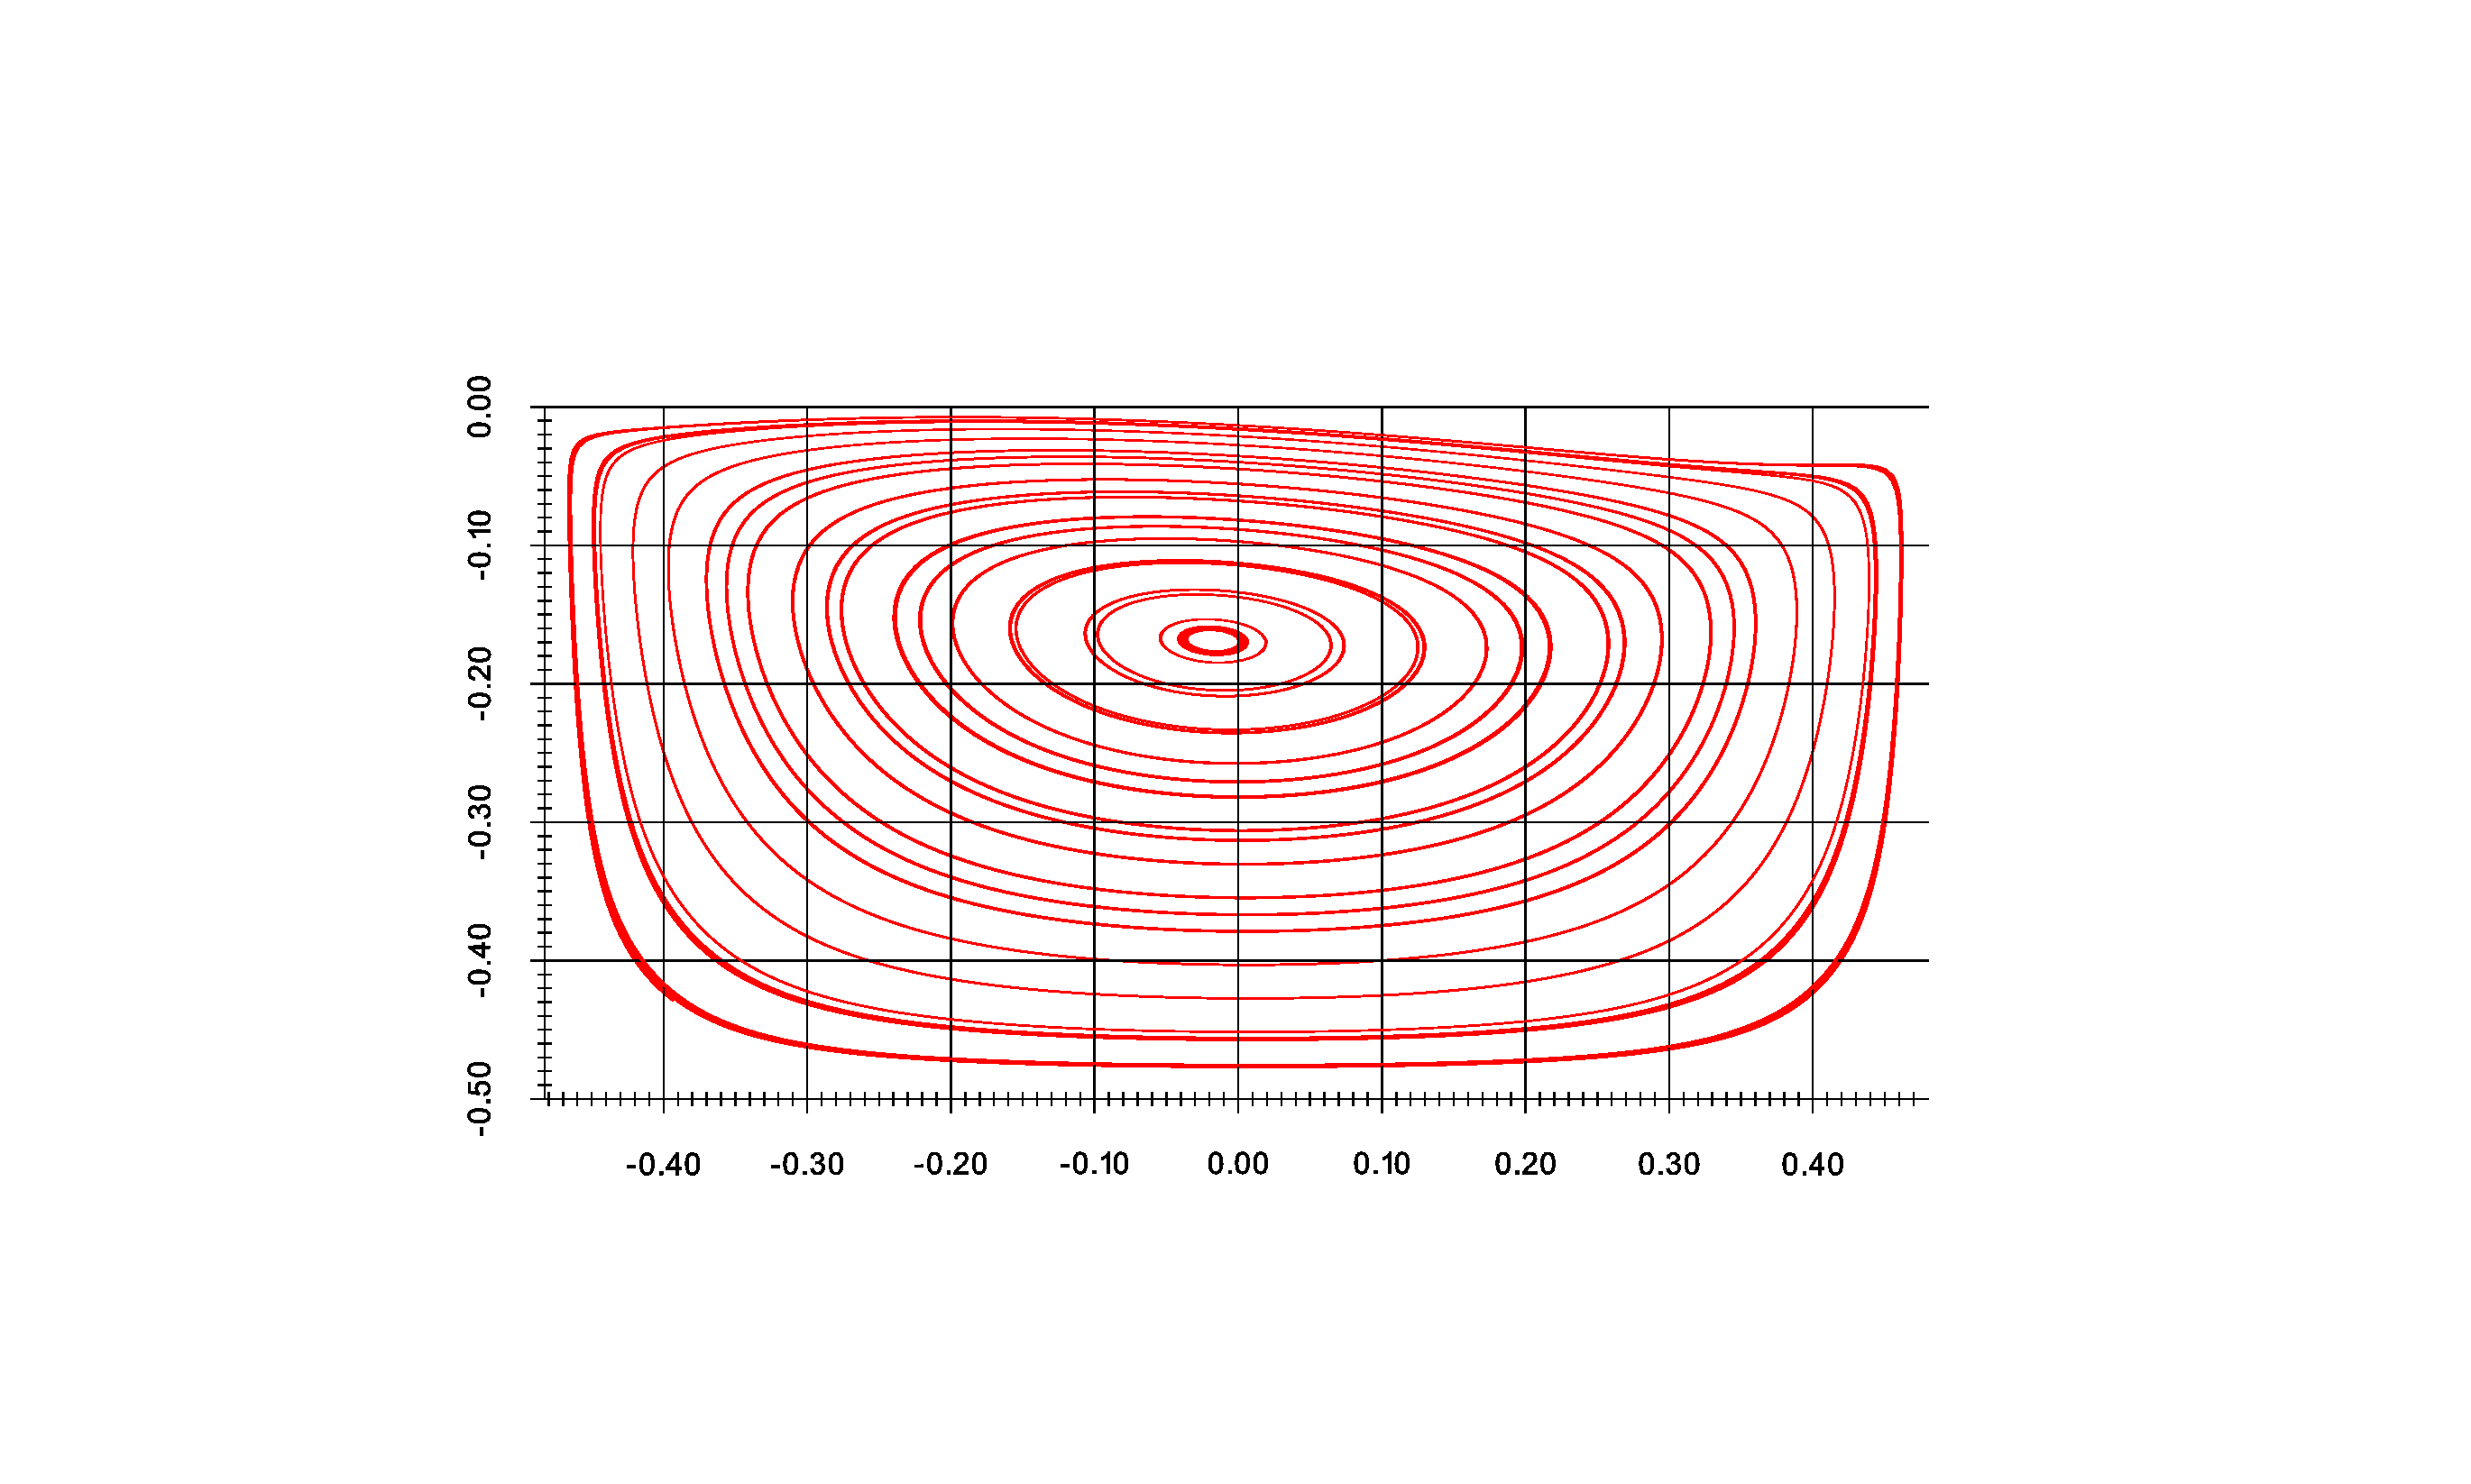
\includegraphics[width=0.5\textwidth]{figure/AR0.5-Re100 streamFunction axis final.pdf}
\caption{AR=0.5, Re=100 (base case)}
\label{AR0.5RE100}

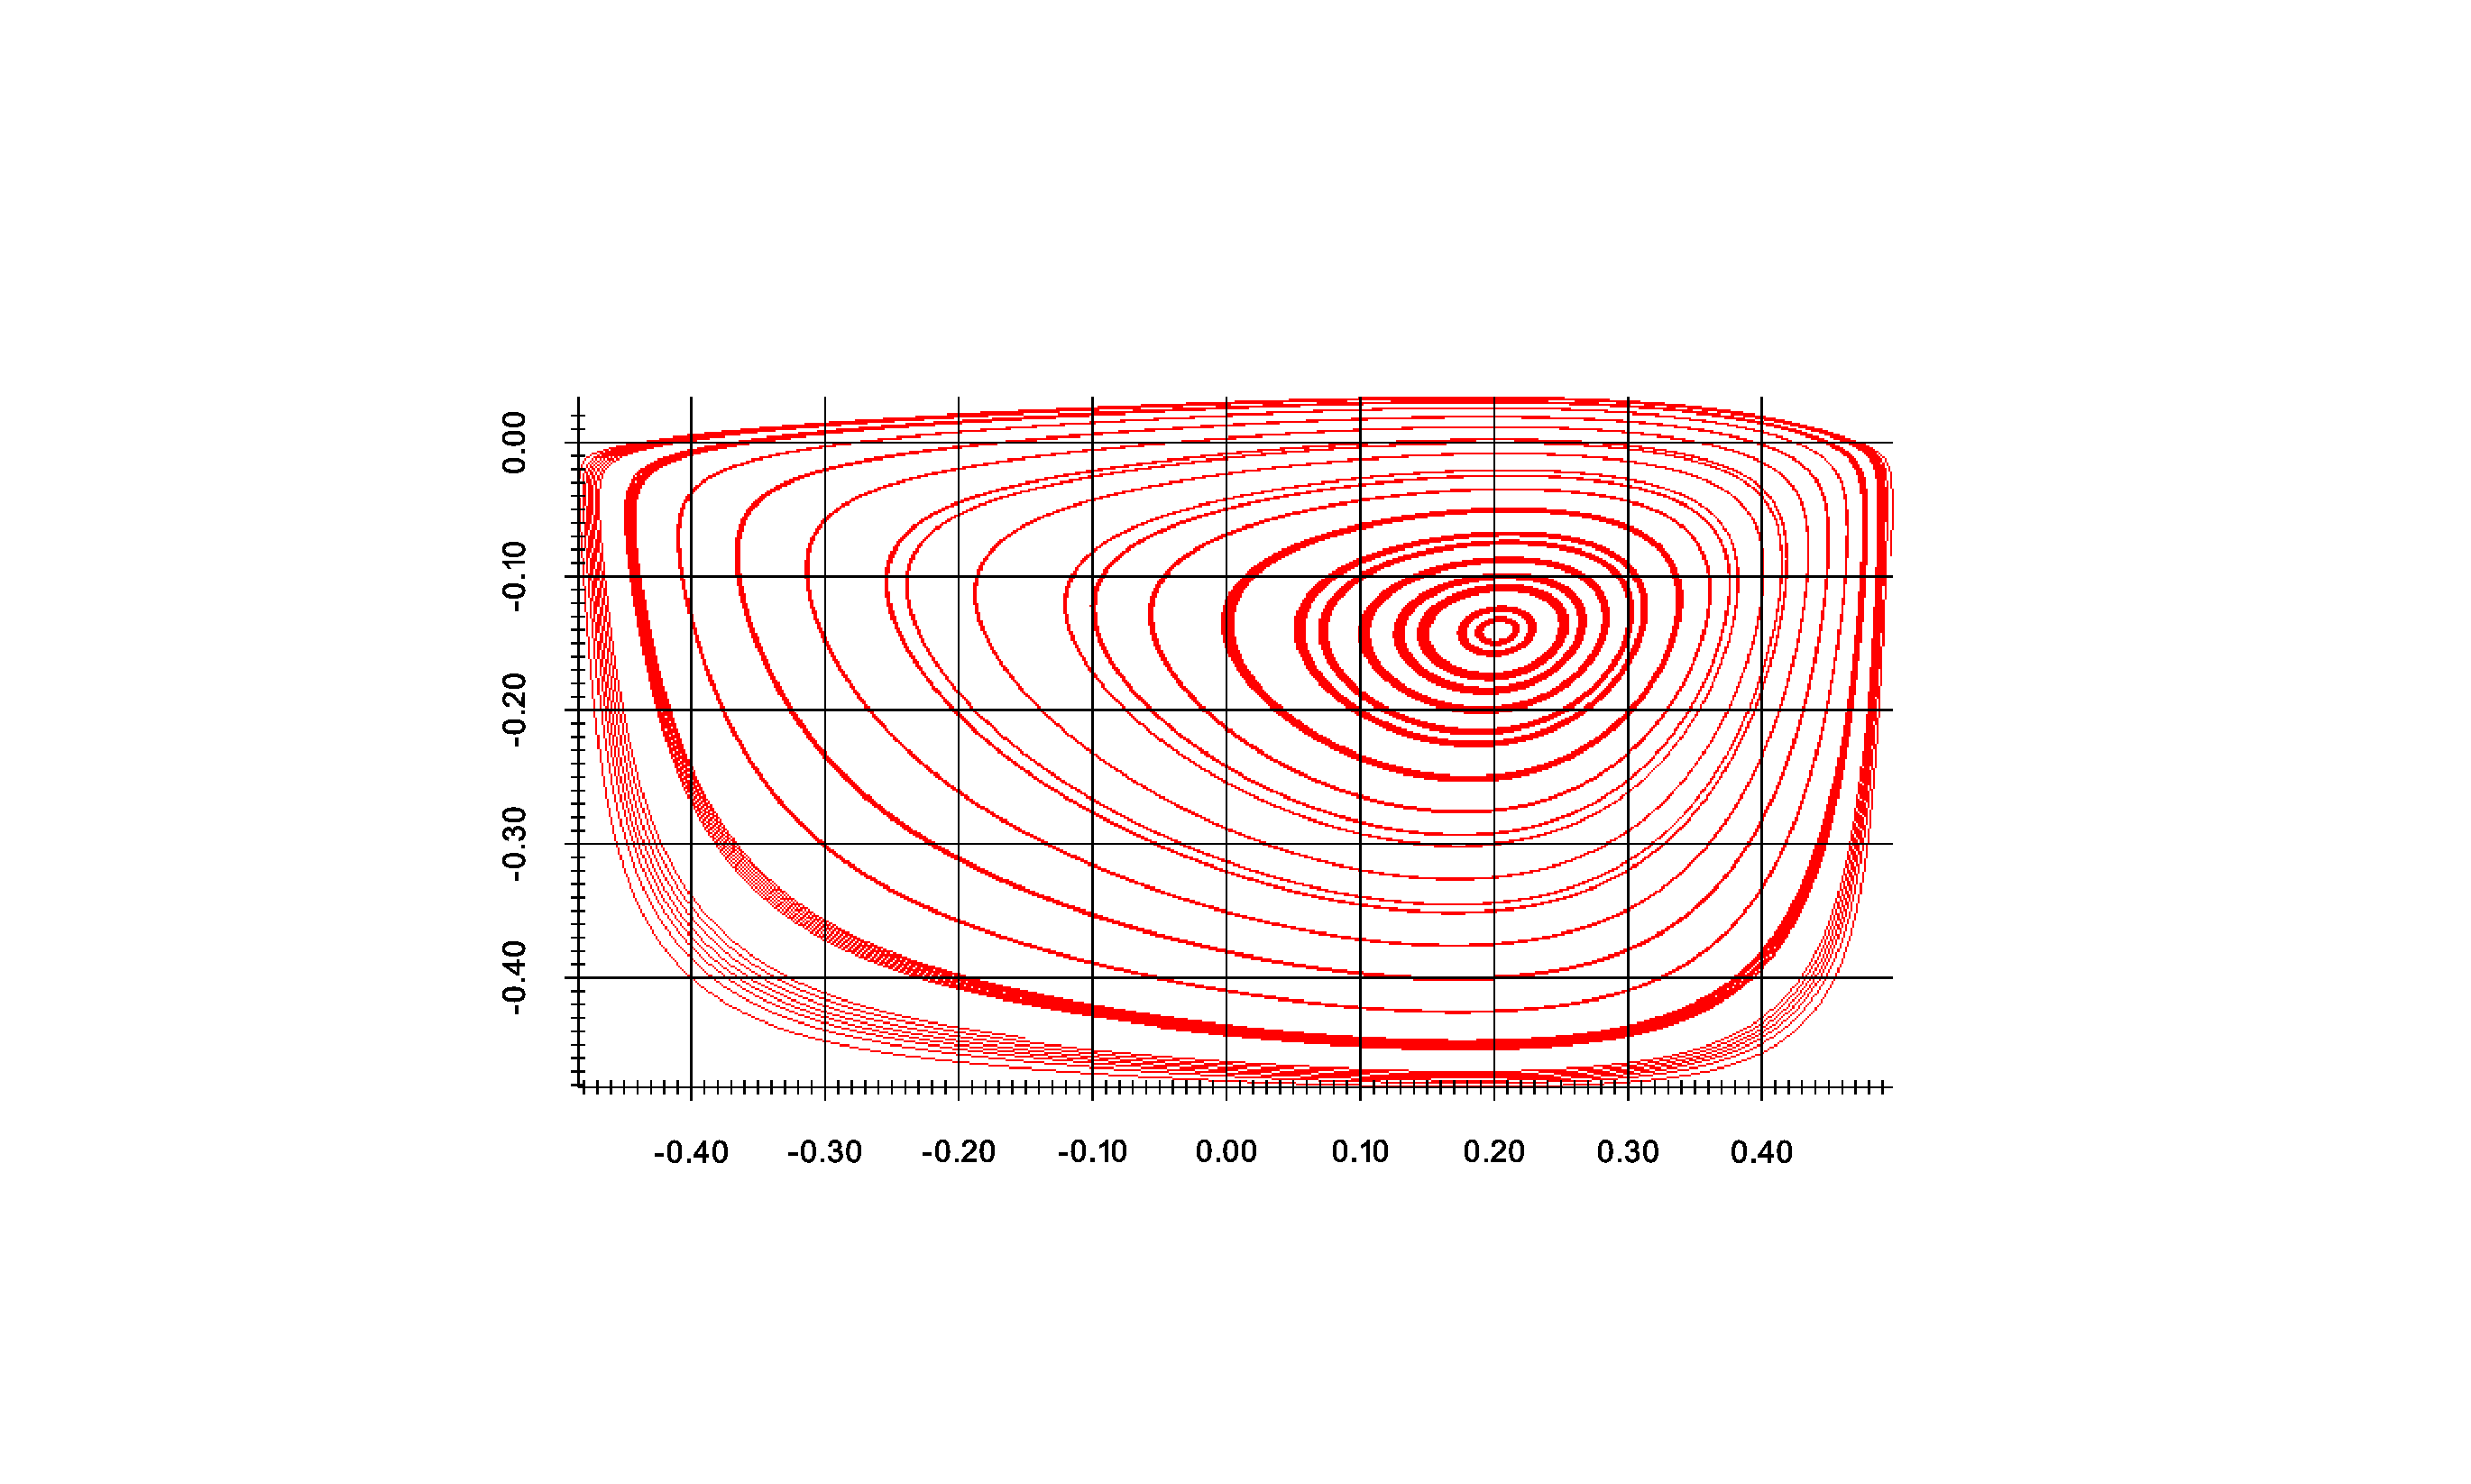
\includegraphics[width=0.5\textwidth]{figure/AR0.5-Re2000 streamFunction axis final.pdf}
\caption{AR=0.5, Re=2000}
\label{AR0.5RE2000}
\end{center}
\end{figure}

%%%%%%%%%%%%%%%%%%%%%%%%%%%%%%%%%%%%%%%%%%%%%%%%%%%%%%%%%%%%%%%%%%%%%%
\section{Conclusion}

%%%%%%%%%%%%%%%%%%%%%%%%%%%%%%%%%%%%%%%%%%%%%%%%%%%%%%%%%%%%%%%%%%%%%%
\nocite{*}
\bibliographystyle{asmems4}
\bibliography{asme2e}

\clearpage
\begin{figure}[tbh]
        \centering
        \begin{subfigure}[b]{0.5\textwidth}
                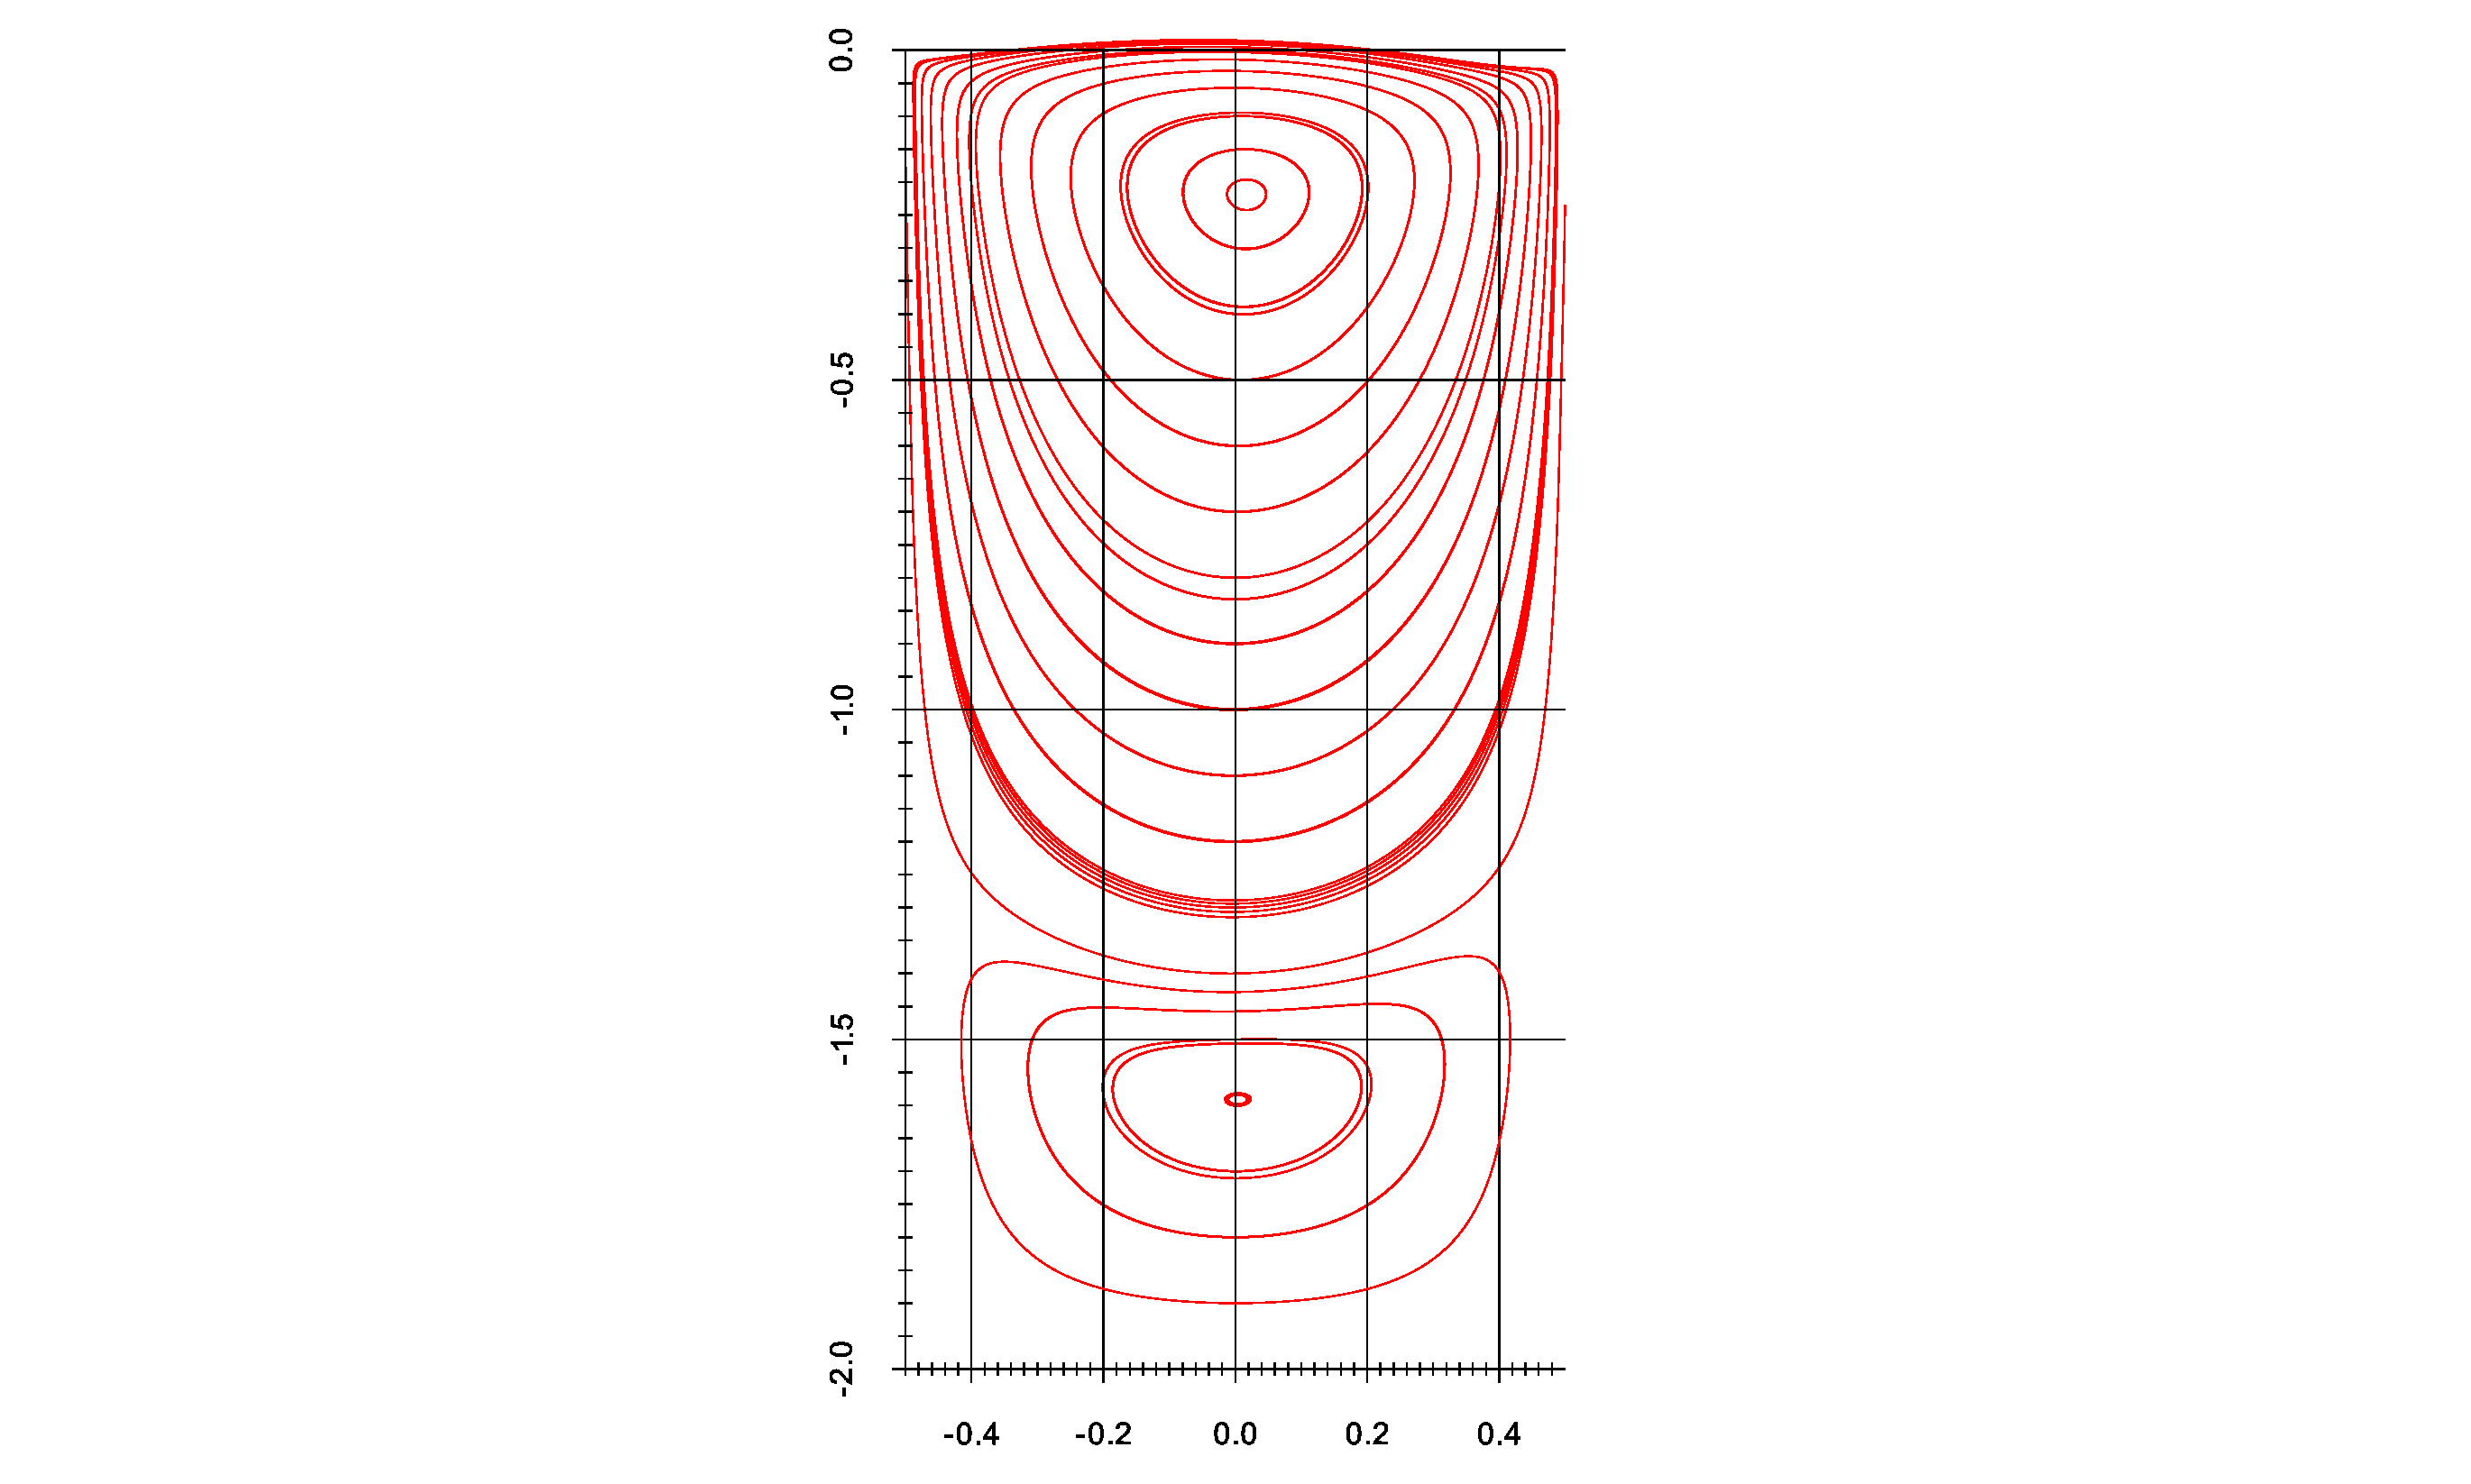
\includegraphics[width=\textwidth]{figure/AR2-Re100 streamFunction axis final.pdf}
                \caption{Cavity eddies}
                \label{AR2RE100_cavity}
        \end{subfigure}%
        \label{AR2RE100}

        \begin{subfigure}[b]{0.22\textwidth}
                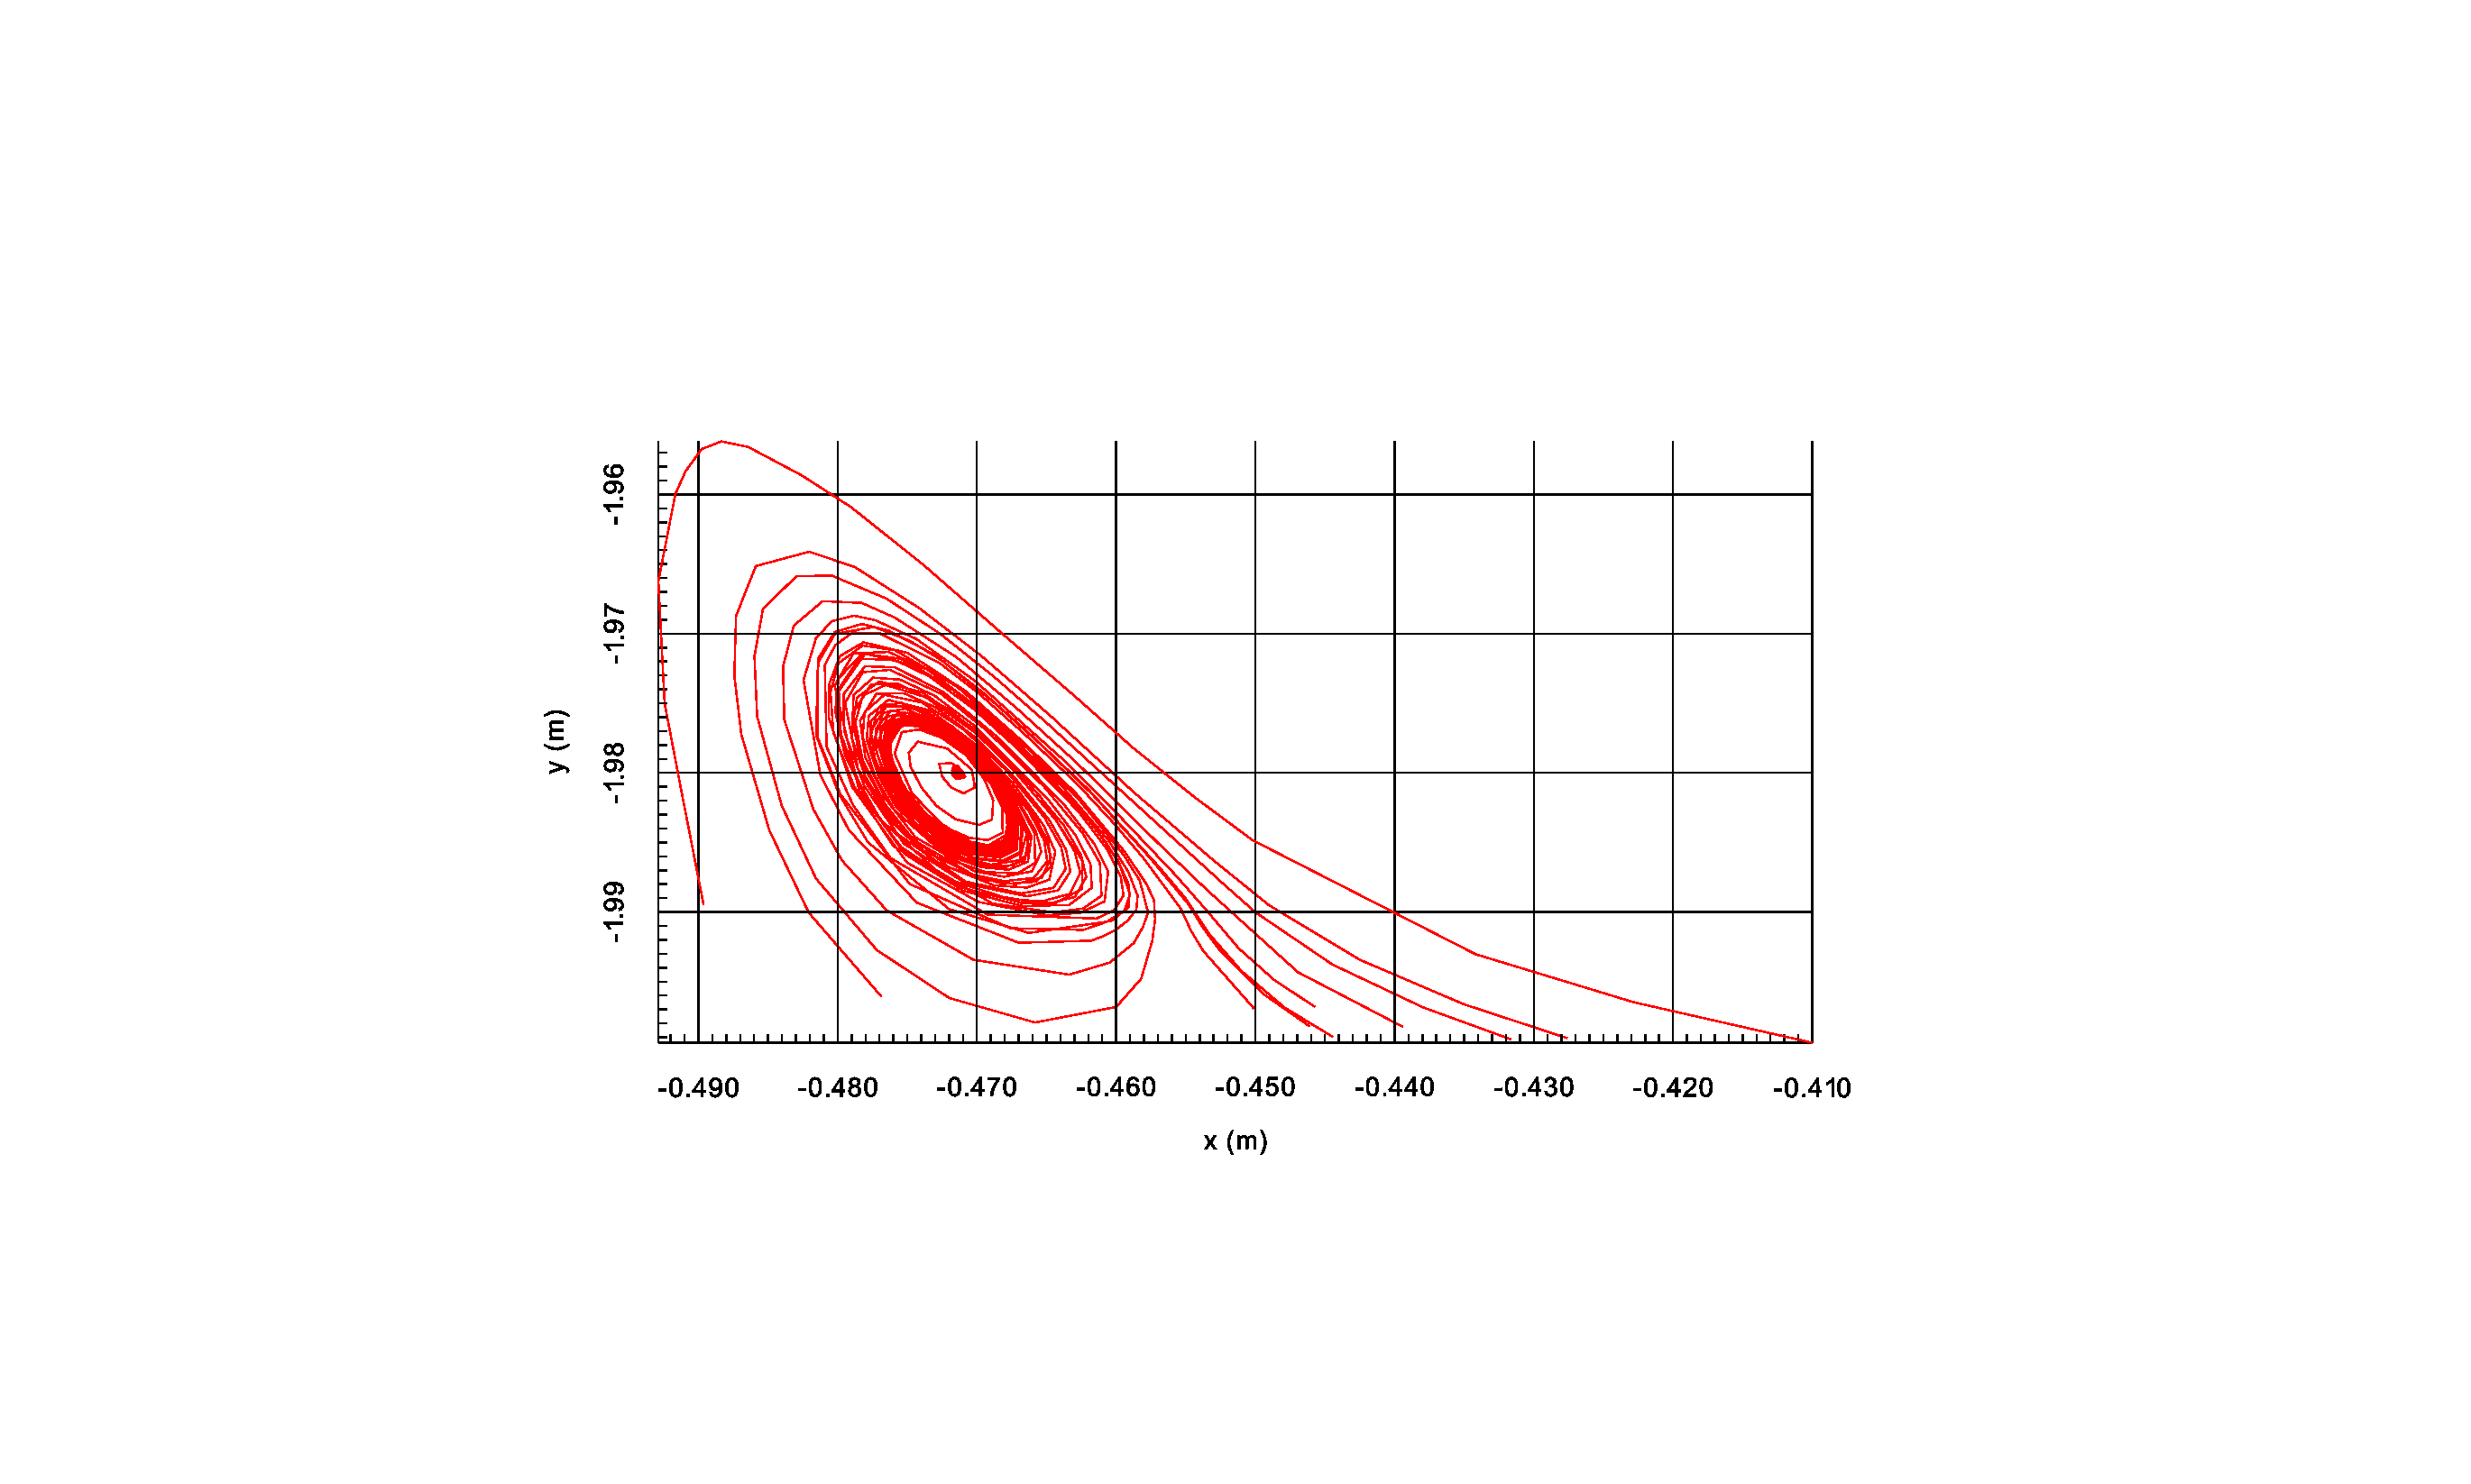
\includegraphics[width=\textwidth]{figure/leftVortex.pdf}
                \caption{Upstream corner eddy, large ticks are 0.01m (y $\in \{-1.94, -2.00\}$, x $\in \{-.50, -.44\}$)}
                \label{AR2RE100_upstream}
        \end{subfigure}%
        \qquad
        \begin{subfigure}[b]{0.22\textwidth}
                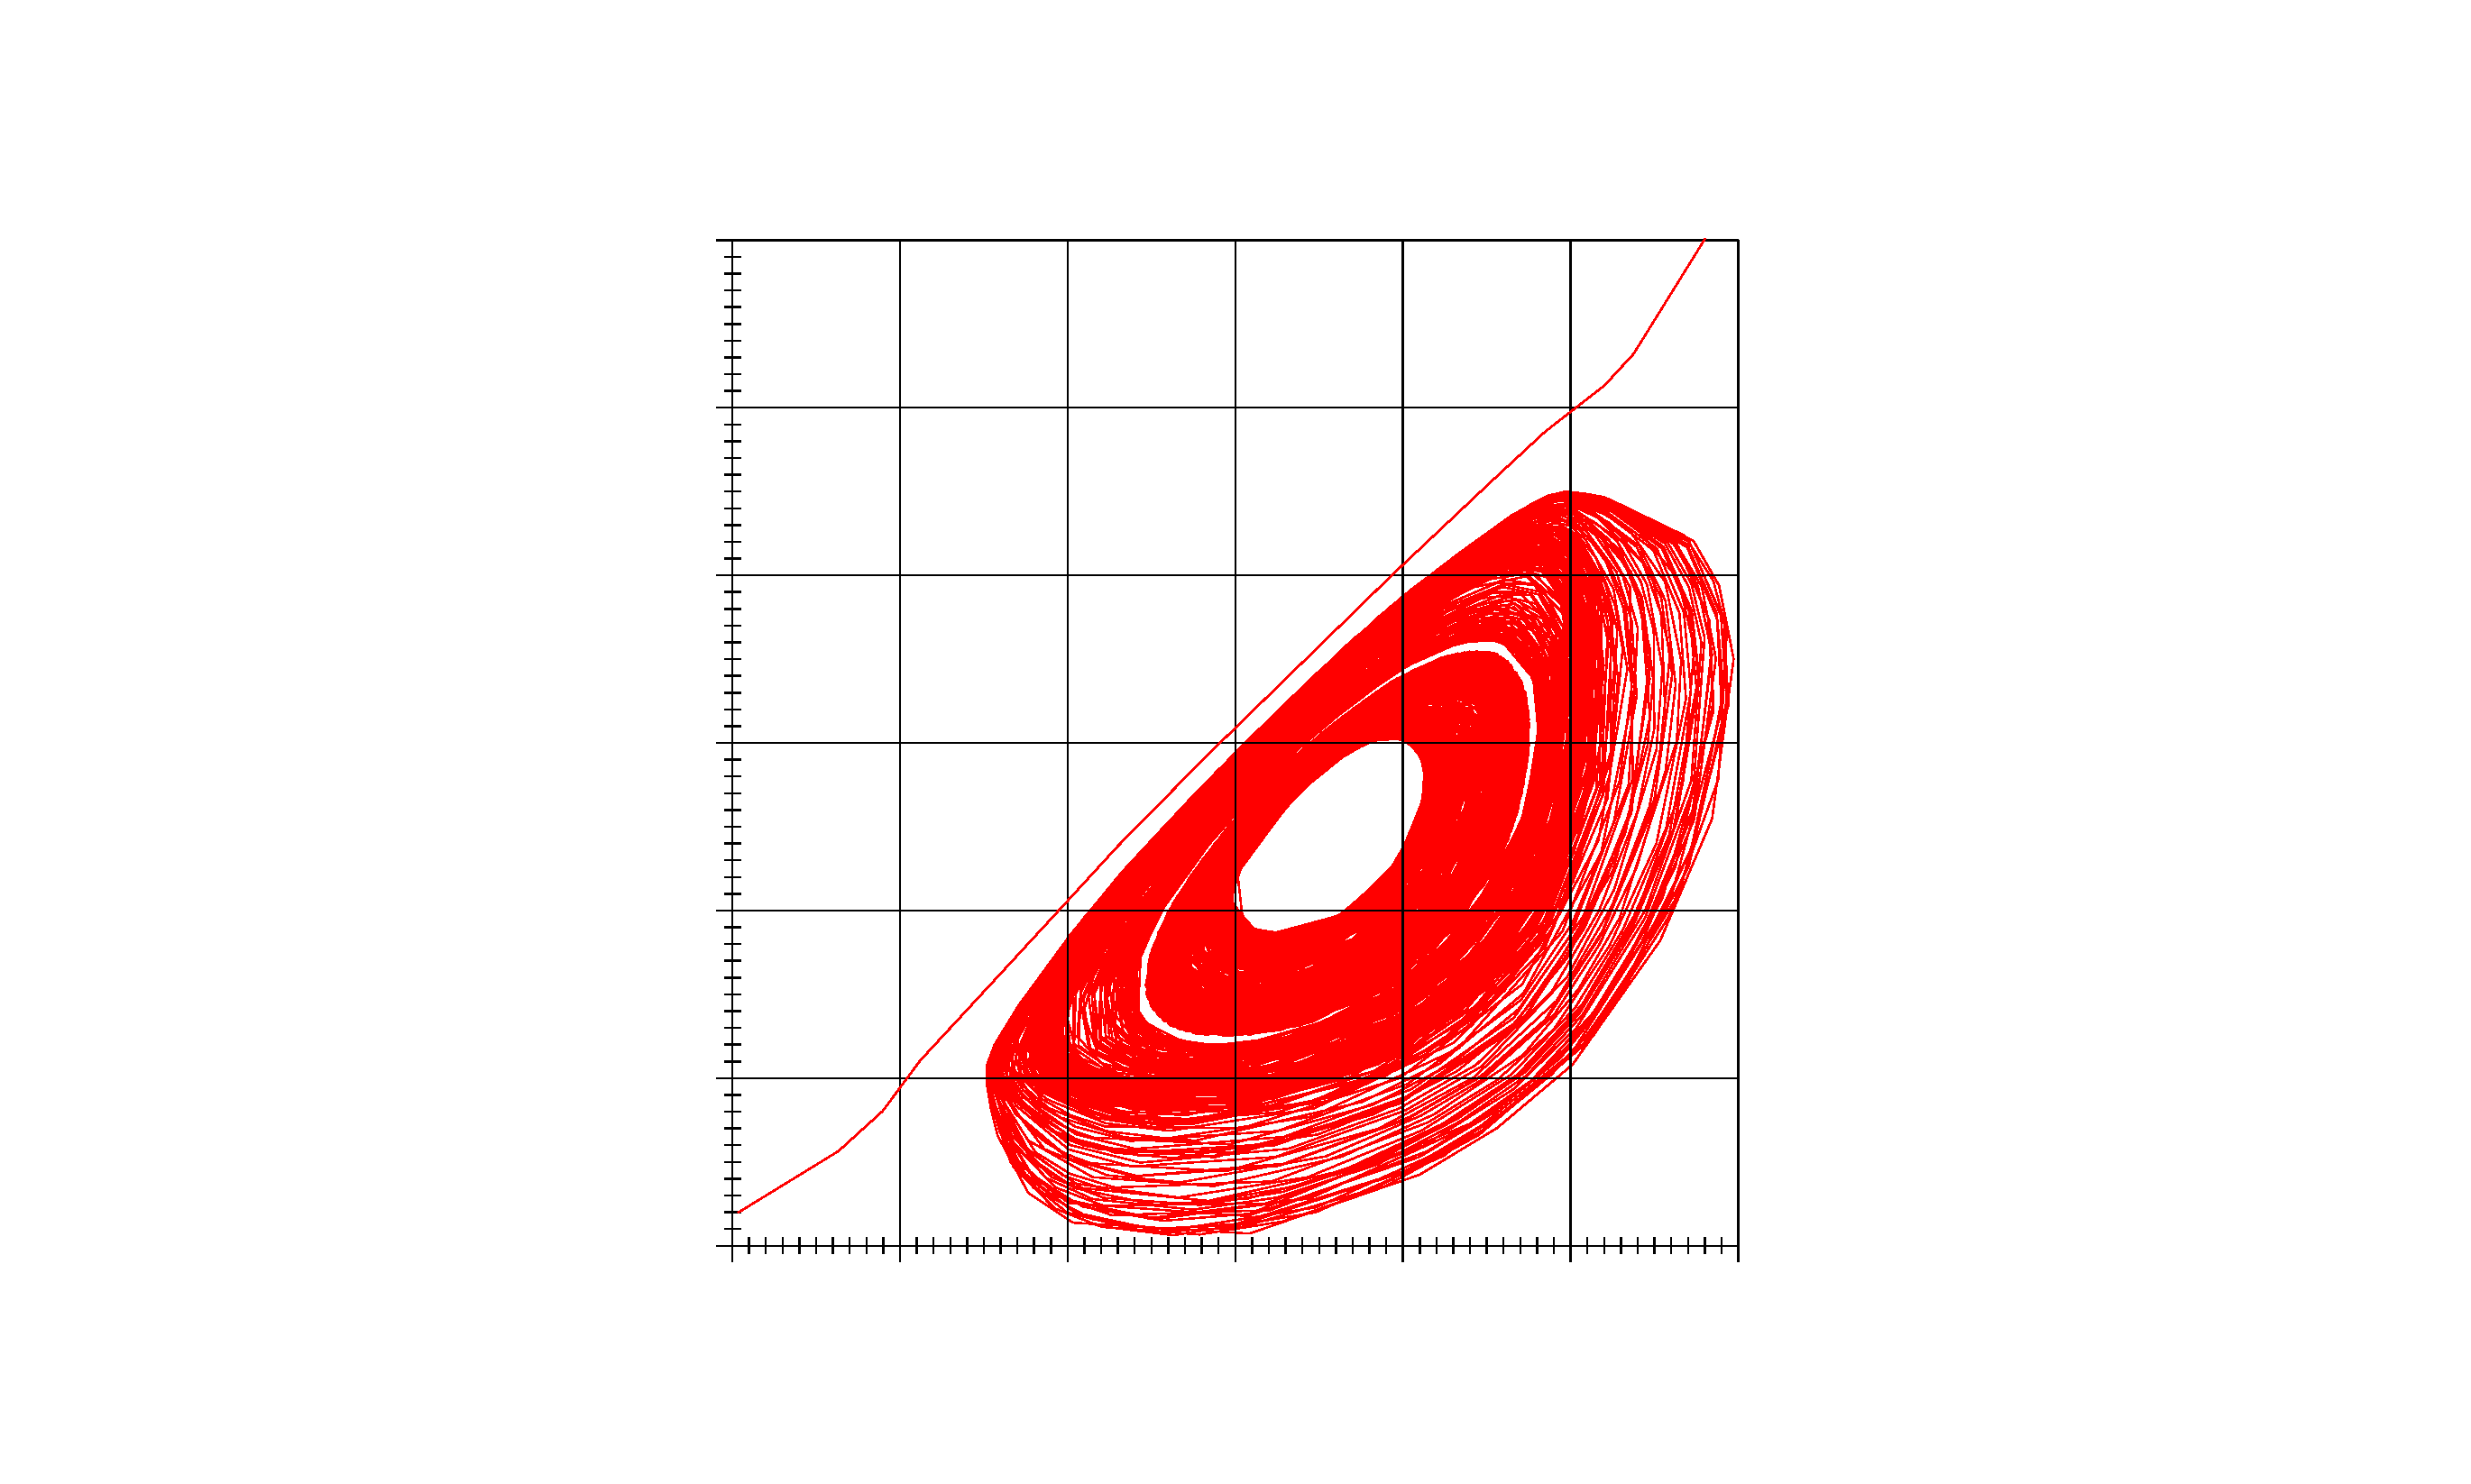
\includegraphics[width=\textwidth]{figure/rightVortex.pdf}
                \caption{Downstream corner eddy, large ticks are 0.01m (y $\in \{-1.94, -2.00\}$, x $\in \{.44, .50\}$)}
                \label{AR2RE100_downstream}
        \end{subfigure}
        \caption{AR=2, Re=100}\label{AR2RE100}

\end{figure}

\begin{figure}[tbh]
\begin{center}
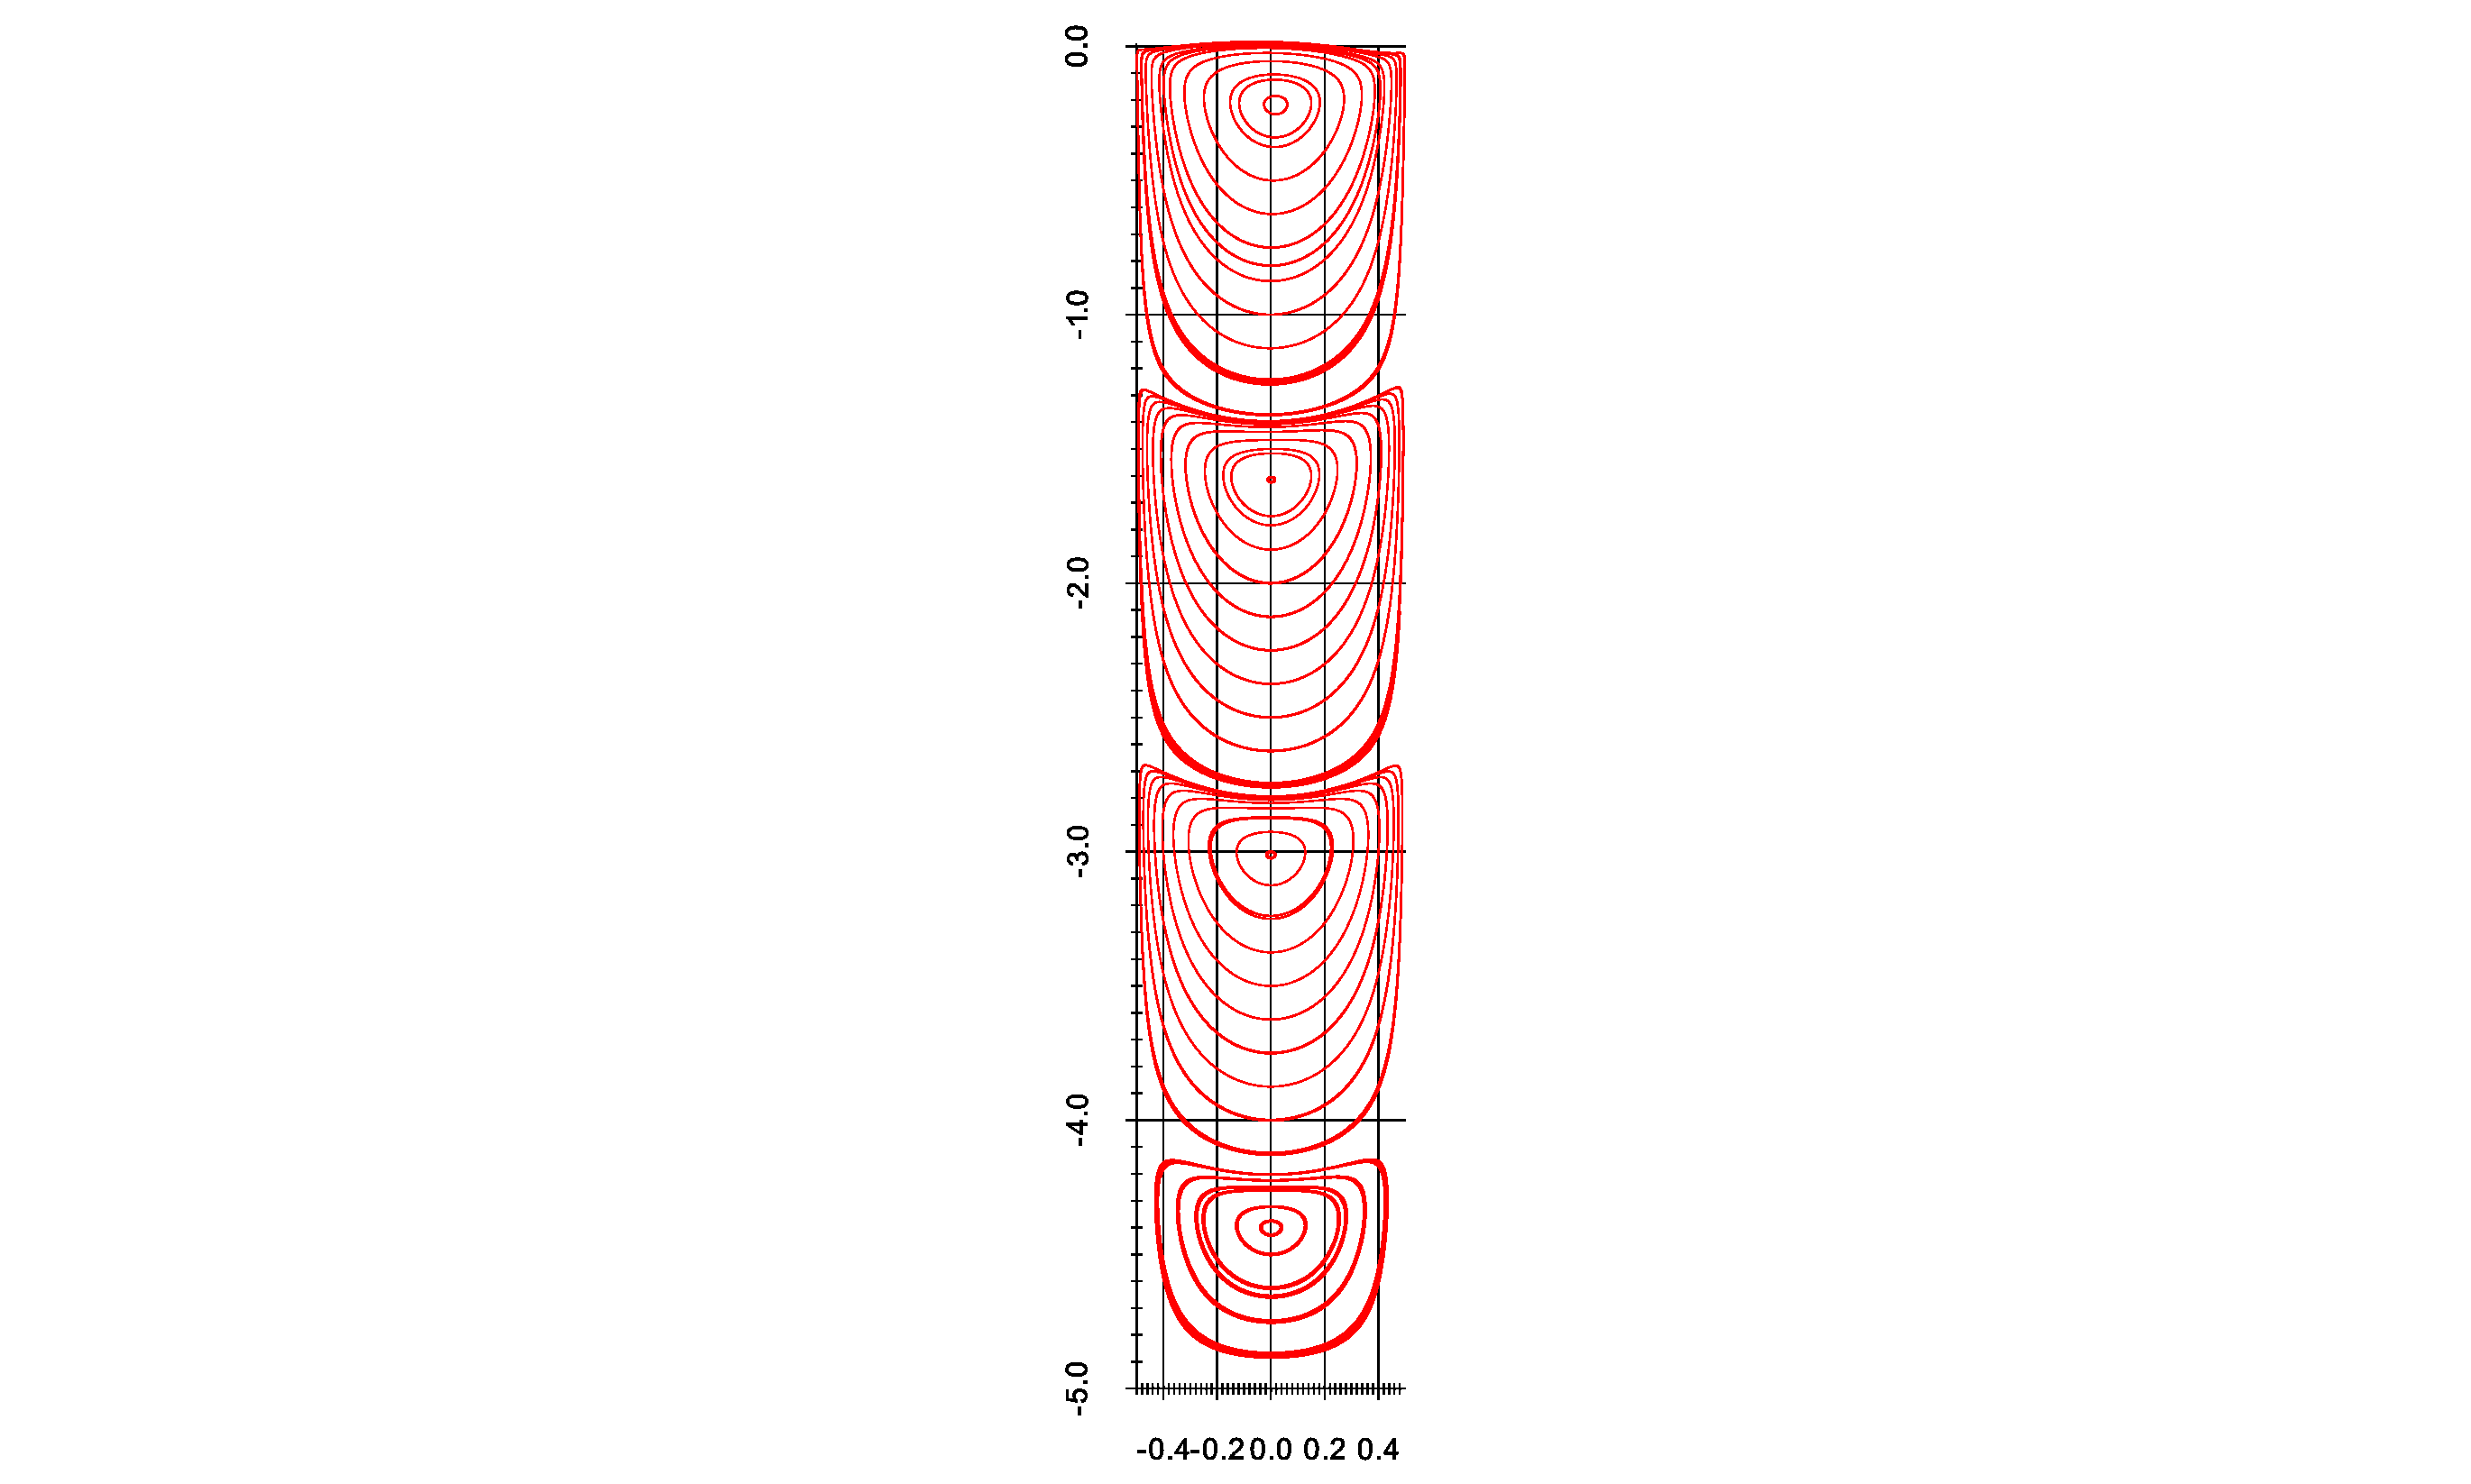
\includegraphics[height=1.4\textwidth]{figure/AR5-Re100 streamFunction axis final.pdf}
\caption{AR=5, Re=100}
\label{}
\end{center}
\end{figure}

%%%%%%%%%%%%%%%%%%%%%%%%%%%%%%%%%%%%%%%%%%%%%%%%%%%%%%%%%%%%%%%%%%%%%%
\clearpage
\onecolumn
\appendix       %%% starting appendix
\section*{Appendix A: Python Code}

\lstinputlisting[caption=Code to create solutions, language=Python]{../code/Final.py}

%%%%%%%%%%%%%%%%%%%%%%%%%%%%%%%%%%%%%%%%%%%%%%%%%%%%%%%%%%%%%%%%%%%%%%
\end{document}
